\documentclass[notitlepage]{article}
%twocolumn for two columns saves space

\usepackage{amsmath}
\usepackage{fullpage}
\usepackage{graphicx}
\usepackage{hyperref}
\usepackage{subcaption}
\usepackage{amsfonts}
\usepackage{booktabs}

\usepackage{parskip}

% https://tex.stackexchange.com/questions/8625/force-figure-placement-in-text
\usepackage{float}

% space saving
\usepackage[text={16cm,24cm}]{geometry}
\usepackage[compact]{titlesec}
\usepackage{mathptmx}

\usepackage[backend=biber,style=ieee,sorting=ynt]{biblatex}
\bibliography{citation}

% https://tex.stackexchange.com/questions/111948/what-is-a-overfull-hbox-9-89561pt-too-wide
\sloppy

\title{IYSE6420: BirdCLEF Birdcall Distribution Maps}

%% Authors
\author{
    Anthony Miyaguchi \texttt{<acmiyaguchi@gatech.edu>}
}

\begin{document}
\maketitle
\thispagestyle{empty}

\begin{abstract}

We utilize geospatial features of bird call metadata from the BirdCLEF 2022 competition to derive a distribution map for a subset of species in California and the Western United States.
We build several Bayesian models incorporating species frequency information and remote sensing data from USGS and NASA in a regular lattice built from area-of-interest (AOI) geometries. 
We use hierarchical modeling to incorporate information across a subset of species and a conditional autoregressive (CAR) distribution for spatial random effects and generate several species distribution maps.
All code and data are available on request and may be available publicly on GitHub/GCP, pending permission from course instructors.

\end{abstract}

\section{Introduction}

We are interested in whether we can produce and analyze species distribution maps using Bayesian methods.

The BirdCLEF Challenge is a yearly competition held as part of the Conference and Labs of the Evaluation Forum.
The purpose of the challenge is to classify bird call segments and species from soundscapes captured from audio recording devices deployed in the fields.
The competition hosts provide a training dataset derived from xeno-canto, a crowd-sourced platform for sharing user-generated recordings of bird calls worldwide.

\section{Dataset}
\subsection{BirdCLEF 2022 Training Metadata}

The BirdCLEF 2022 competition provides over 14,800 recordings from 152 species \cite{kahl2022overview}.
We are interested in the spatial features from the recording metadata, which are the latitude and longitude of the recording.
The competition draws recordings from the xeno-canto library, but it does not reflect the entirety of the library.
Each species is capped at 500 recordings in the dataset, with the frequency of recordings generally correlated with their rarity in nature and population density, among other factors.

\subsection{Google Earth Engine}

Google Earth Engine is a cloud-based platform for processing geospatial data \cite{gorelick_google_2017}.
We use remote sensing data from the United States Geological Survey (USGS) and the National Aeronautics and Space Administration (NASA) to obtain elevation, temperature, land cover classification, and population density data from various sources hosted on Earth Engine.

The NASA Shuttle Radar Topography Mission dataset (\texttt{USGS/SRTMGL1\_003}) \cite{nasa_srtmg} provides elevation data.
The TMODIS/Terra Land Surface Temperature/Emissivity dataset (\texttt{MODIS/006/MOD11A1}) \cite{wan_zhengming_mod11a1_2015} provides temperature data.
The MODIS/Terra+Aqua Land Cover Type dataset (\texttt{MODIS/006/MCD12Q1}) \cite{friedl_mark_mcd12q1_2019} provides land cover classification statistics.
The Gridded Population of the World, Version 4 dataset (\texttt{CIESIN/GPWv411/GPW\_Population\_Density}) \cite{gpwv4} provides population density data.

We generate a regular lattice of polygons from area-of-interest (AOI) geometries that derive a dataset for a region at a fraction of a degree resolution.
We chose California and the Western United States as our AOI due to familiarity with the region and the diversity of geography and climate.
The dataset is generated over each polygon in the lattice, computing an aggregate statistic from each data source.

\section{Data and Analysis}

\subsection{Conditional Autoregressive Distribution}

The likelihood for a conditional autoregression (CAR) distribution is given by the following equation:

\begin{equation}
f(x|W, \alpha, \tau) =
    \frac{|T|^{1/2}}{(2\pi)^{k/2}}
    \exp \left\{
        -\frac{1}{2} (x - \mu)^\prime T^{-1} (x - \mu)
    \right\}
\end{equation}

where

\begin{equation}
\begin{aligned}
    T &= (\tau D (I-\alpha W))^{-1} \\
    D &= diag(\sum_{i} W_{ij})
\end{aligned}
\end{equation}


This is a special form of the multivariate normal with with a covariance matrix that captures the adjacency structure of the neighborhood graph. 
PyMC provides this distribution out-of-the-box, which we utilize for spatial random effects \cite{salvatier_probabilistic_2016}.

\subsection{Stochastic Search Variable Selection}

There are a total of 27 features that are available for modeling.
Many of these features, such as land cover classification, may have a significant degree of skewness affecting the fitted model.
We use a stochastic search variable selection (SSVS) to inform our choice of feature transformation.

\begin{figure}[H]
\centering
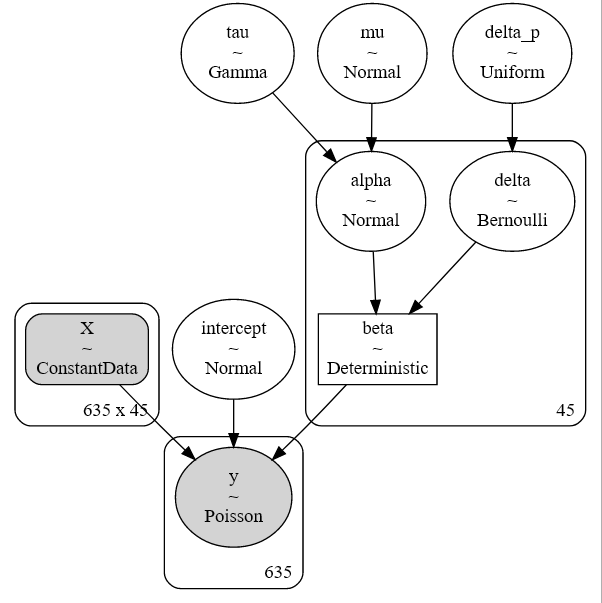
\includegraphics[width=0.5\textwidth]{report/figures/svss_model.png}
\end{figure}

We fit a Poisson GLM to the Western US dataset where $\beta$ terms are a deterministic function $\delta$ representing the binary likelihood that a co-variate is included in the model and $\alpha$ representing the strength of the co-variate in the regression.
In our first model, we include all of the raw (or non-transformed) features and concatenate it with the log-scaled features of population density and land cover classification.
We do not scale elevation and temperature because these features are not heavy tailed.

\begin{figure}[hbt!]
\centering
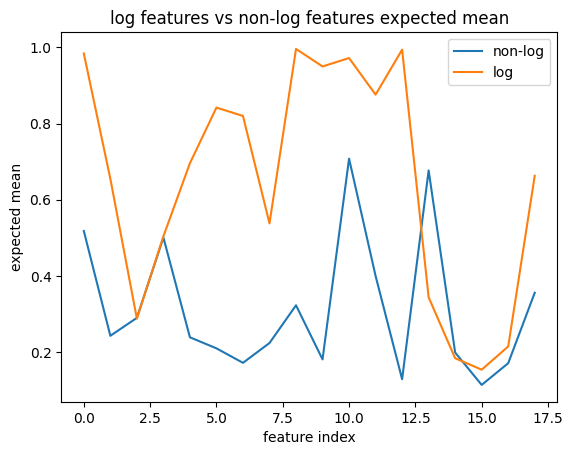
\includegraphics[width=0.6\textwidth]{report/figures/svss_log_vs_nonlog_features.png}
\caption{A comparison of non-transformed and transformed features.}
\label{fig:svss_log_vs_nonlog}
\end{figure}

\begin{figure}[H]
\centering
\begin{tabular}{llr}
\toprule
{} &                                        feature &  probability \\
\midrule
0 &  000010110000000000010010000100011001111100000 &     0.000450 \\
1 &  100010110000000000000000000100010101111100001 &     0.000425 \\
2 &  100010110000000000000000000100011101111100001 &     0.000350 \\
3 &  000010110000000000000010000100011101111100001 &     0.000325 \\
4 &  000011010000000000000000000110011001111100000 &     0.000250 \\
\bottomrule
\end{tabular}
\caption{Top models with Poisson GLM with non-transformed and log-scaled co-variates. Each string represents a binary mask for whether a feature is included in a model. The first 27 positions are non-transformed, while the last 18 are log-transformed.}
\label{table:svss_log_vs_nonlog_models}
\end{figure}

We observe in figure \ref{fig:svss_log_vs_nonlog} that mean values of $\delta$ are larger, and therefore more likely to be included in a model.
We count the instances of each possible model and find the most likely models supported by the data.
In table \ref{table:svss_log_vs_nonlog_models}, we find that the SSVS procedure favors log-scaled land cover classification features over the non-transformed features.
This corroborates the comparison of $\delta$ means in figure \ref{fig:svss_log_vs_nonlog}.

\begin{figure}[H]
\centering
\begin{tabular}{lrrrrl}
\toprule
{} &   mean &     sd &  hdi\_3\% &  hdi\_97\% &        feature\_name \\
\midrule
delta[0]  &  0.993 &  0.084 &     1.0 &      1.0 &  population\_density \\
delta[1]  &  0.674 &  0.469 &     0.0 &      1.0 &        elevation\_p5 \\
delta[2]  &  0.601 &  0.490 &     0.0 &      1.0 &       elevation\_p50 \\
delta[3]  &  0.619 &  0.486 &     0.0 &      1.0 &       elevation\_p95 \\
delta[4]  &  1.000 &  0.000 &     1.0 &      1.0 &      LST\_Day\_1km\_p5 \\
delta[5]  &  0.857 &  0.350 &     0.0 &      1.0 &     LST\_Day\_1km\_p50 \\
delta[6]  &  0.733 &  0.442 &     0.0 &      1.0 &     LST\_Day\_1km\_p95 \\
delta[7]  &  1.000 &  0.000 &     1.0 &      1.0 &    LST\_Night\_1km\_p5 \\
delta[8]  &  0.651 &  0.477 &     0.0 &      1.0 &   LST\_Night\_1km\_p50 \\
delta[9]  &  0.588 &  0.492 &     0.0 &      1.0 &   LST\_Night\_1km\_p95 \\
delta[10] &  0.991 &  0.094 &     1.0 &      1.0 &       land\_cover\_01 \\
delta[11] &  0.478 &  0.500 &     0.0 &      1.0 &       land\_cover\_02 \\
delta[12] &  0.778 &  0.416 &     0.0 &      1.0 &       land\_cover\_03 \\
delta[13] &  0.975 &  0.158 &     1.0 &      1.0 &       land\_cover\_04 \\
delta[14] &  0.983 &  0.130 &     1.0 &      1.0 &       land\_cover\_05 \\
delta[15] &  0.932 &  0.253 &     0.0 &      1.0 &       land\_cover\_06 \\
delta[16] &  0.879 &  0.326 &     0.0 &      1.0 &       land\_cover\_07 \\
delta[17] &  1.000 &  0.000 &     1.0 &      1.0 &       land\_cover\_08 \\
delta[18] &  0.991 &  0.095 &     1.0 &      1.0 &       land\_cover\_09 \\
delta[19] &  0.892 &  0.311 &     0.0 &      1.0 &       land\_cover\_10 \\
delta[20] &  1.000 &  0.007 &     1.0 &      1.0 &       land\_cover\_11 \\
delta[21] &  1.000 &  0.000 &     1.0 &      1.0 &       land\_cover\_12 \\
delta[22] &  0.708 &  0.455 &     0.0 &      1.0 &       land\_cover\_13 \\
delta[23] &  0.388 &  0.487 &     0.0 &      1.0 &       land\_cover\_14 \\
delta[24] &  0.480 &  0.500 &     0.0 &      1.0 &       land\_cover\_15 \\
delta[25] &  0.422 &  0.494 &     0.0 &      1.0 &       land\_cover\_16 \\
delta[26] &  0.972 &  0.165 &     1.0 &      1.0 &       land\_cover\_17 \\
\bottomrule
\end{tabular}
\caption{Probability that a feature is included in a model via SSVS. We note that population density and land cover classification features are log-scaled.}
\label{table:delta_values}
\end{figure}

\begin{figure}[H]
\centering
\begin{tabular}{llr}
\toprule
{} &                      feature &  probability \\
\midrule
0 &  111111111111111111111111111 &     0.050600 \\
1 &  111111111111111111111110111 &     0.013237 \\
2 &  111111111111111111111111011 &     0.012725 \\
3 &  111111111111111111111111101 &     0.009838 \\
4 &  111111111110111111111111111 &     0.008563 \\
\bottomrule
\end{tabular}
\caption{Top models with Poisson GLM with non-transformed elevation and temperature features, and log-scaled population density and land cover classification features.}
\label{table:svss_model}
\end{figure}

We provide the full summary of $\delta$ posteriors in table \ref{table:delta_values}.
We also provide the most likely models in table \ref{table:svss_model}.
We choose the set of non-transformed elevation and temperature features with log-scaled population density and land cover classification features for our final model. 

\subsection{Model Selection}
\label{model_selection}

We try out a variety of Poisson Generalized Linear Models (GLMs) for developing our distribution map.
There are three main components to these models: an intercept term, a feature term, and a random spatial effects term.
We take advantage of hierarchical and multi-level modeling techniques to both pool and vary information across observations, species, and geographical grid indices.

TODO: write out three models

\begin{figure}[H]
\centering
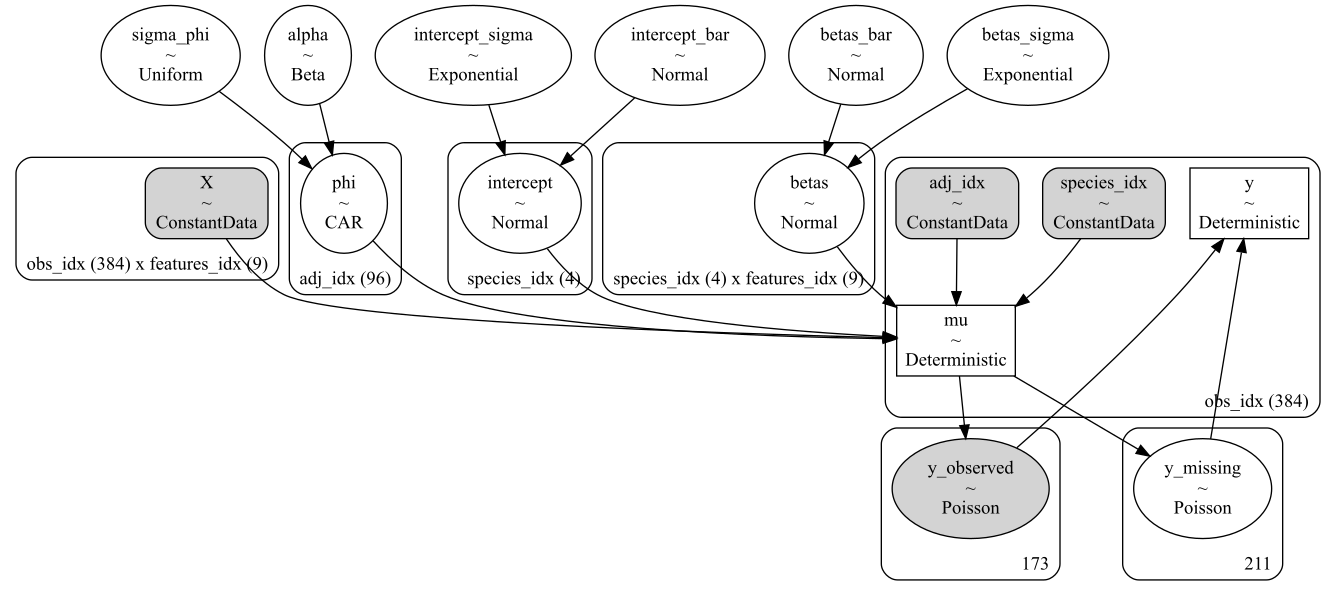
\includegraphics[width=\textwidth]{report/figures/full_model.png}
\caption{Varying intercept, varying covariate, CAR model}
\end{figure}

We compare our models using the widely applicable information criterion (WAIC) on a deviance scale in table \ref{table:waic_comparison}.
We choose the model with the smallest deviance to impute empty cells.
The best model according to the ranking is the varying intercept, varying slope, and CAR model.

\begin{figure}[H]
\centering
\begin{tabular}{lrrrrrr}
\toprule
model\_name &  rank &  elpd\_waic &  p\_waic &  elpd\_diff &      se &     dse \\
\midrule
varying\_intercept\_varying\_slope\_car\_model &     0 &     967.05 &  108.07 &       0.00 &   29.64 &    0.00 \\
pooled\_intercept\_varying\_slope\_car\_model  &     1 &    1237.93 &  198.19 &     270.88 &   54.20 &   44.13 \\
varying\_intercept\_pooled\_slope\_car\_model  &     2 &    1291.85 &  160.71 &     324.80 &  129.09 &  118.68 \\
varying\_intercept\_car\_model                   &     3 &    1296.86 &  163.01 &     329.81 &  129.58 &  119.23 \\
varying\_intercept\_varying\_slope\_model     &     4 &    1748.39 &  307.34 &     781.34 &  155.76 &  149.82 \\
pooled\_intercept\_varying\_slope\_model      &     5 &    1986.66 &  376.32 &    1019.61 &  182.03 &  175.32 \\
varying\_intercept\_pooled\_slope\_model      &     6 &    2094.71 &  292.58 &    1127.66 &  270.45 &  261.44 \\
pooled\_intercept\_car\_model                    &     7 &    3384.61 &  634.20 &    2417.56 &  430.55 &  418.98 \\
pooled\_intercept\_pooled\_slope\_model       &     8 &    3896.91 &  631.80 &    2929.86 &  536.62 &  526.20 \\
varying\_intercept\_model                       &     9 &    4021.92 &  115.95 &    3054.87 &  799.54 &  792.66 \\
\bottomrule
\end{tabular}
\caption{Comparison of models using WAIC on a deviance scale. Lower is better.}
\label{table:waic_comparison}
\end{figure}

\subsection{Posterior Predictive Distribution Maps}

We fit our best model to the data and impute all empty cells in the Western US (2-degree resolution) dataset.
We prepare the dataset by grouping birdcall recording locations into their bounding cells and primary species labels.
To avoid excess computation and sparsity, we choose a subset of bird species and set a default category of "other".

We model using two variations of the prepared dataset.
In figure \ref{fig:map_4}, we choose the top 3 species and impute the rest of the missing cells.
We note that this results in a total of $211/384$ or 55\% of entries that need to be imputed.
Sampling from the posterior takes 7 minutes and 40 seconds with 16 cores for 56000 samples.
The second model uses the top 15 species to generate the dataset, which has greater sparsity with $1178/1536$ or 77\% of entries that need to be imputed.
With greater sparsity comes higher computational costs, with the larger dataset and model taking 37 minutes and 44 seconds to sample.

\begin{figure}[H]
\centering
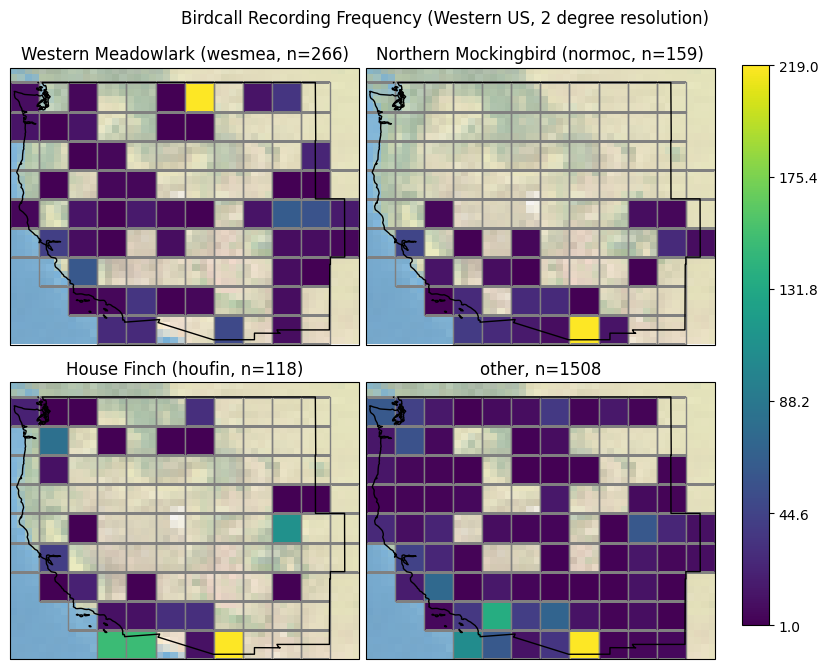
\includegraphics[width=0.8\textwidth]{report/figures/western_us_raw_4.png}
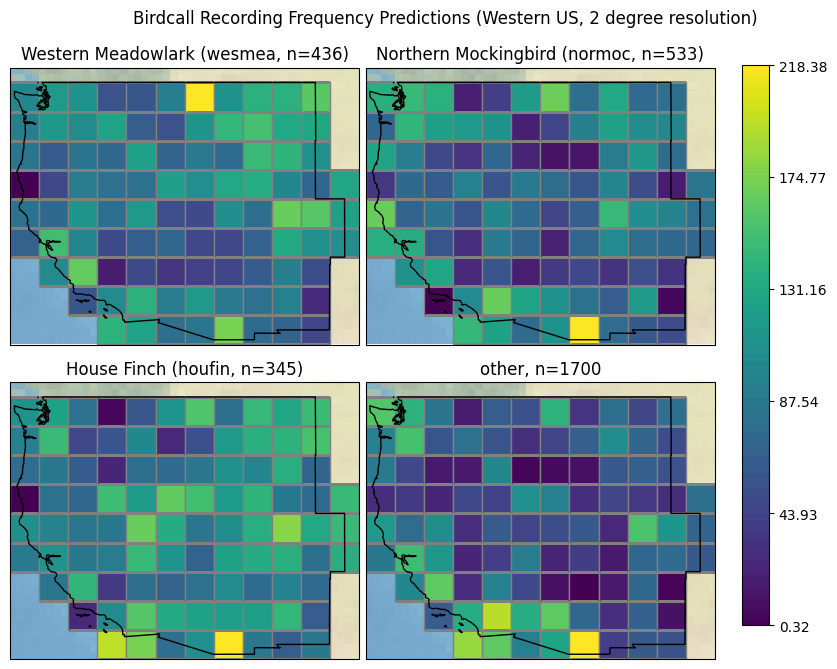
\includegraphics[width=0.8\textwidth]{report/figures/western_us_predict_4.png}
\caption{Frequency maps of the 15 most frequent species.}
\label{fig:map_4}
\end{figure}

\begin{figure}[H]
\centering
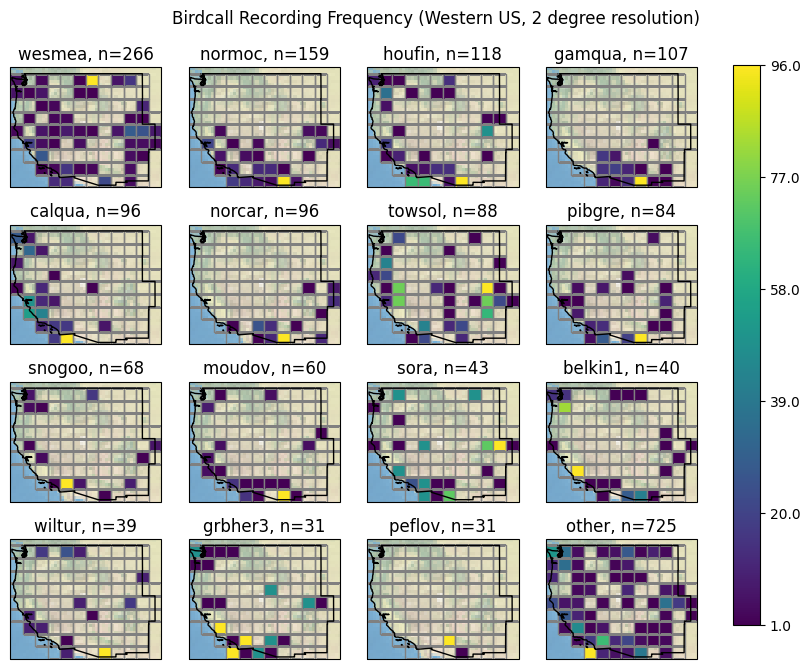
\includegraphics[width=0.8\textwidth]{report/figures/western_us_raw_16.png}
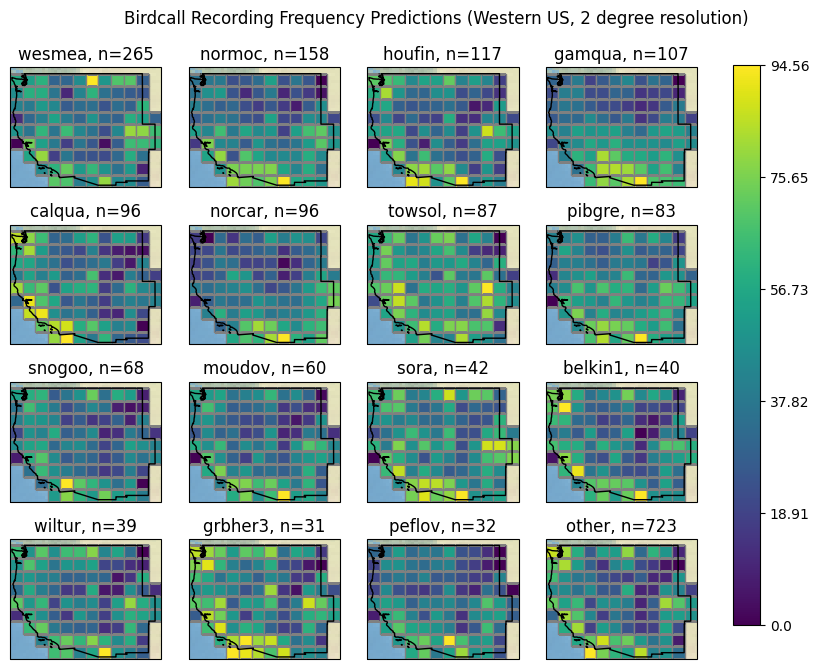
\includegraphics[width=0.8\textwidth]{report/figures/western_us_predict_16.png}
\caption{Frequency maps of the 15 most frequent species.}
\label{fig:map_16}
\end{figure}


\begin{figure}[H]
\centering
\begin{tabular}{lrrrr}
\toprule
\begin{tabular}{lrrrr}
\toprule
index &   mean &     sd &  hdi\_3\% &  hdi\_97\% \\
\midrule
betas[other, landcover\_evergreen\_broadleaf\_forest] &  0.371 &  0.156 &   0.083 &    0.668 \\
betas[other, landcover\_mixed\_forests]              & -0.391 &  0.195 &  -0.756 &   -0.026 \\
betas[other, landcover\_grasslands]                 & -0.440 &  0.186 &  -0.797 &   -0.092 \\
betas[other, landcover\_urban\_and\_built-up]         &  0.664 &  0.228 &   0.239 &    1.094 \\
betas[other, landcover\_cropland/natural\_vegetat... &  0.330 &  0.125 &   0.088 &    0.559 \\
betas[other, landcover\_permanent\_snow\_and\_ice]     &  0.274 &  0.132 &   0.029 &    0.526 \\
betas[other, landcover\_water\_bodies]               &  0.385 &  0.159 &   0.079 &    0.674 \\
\bottomrule
\end{tabular}
\caption{A subset of random slopes from the top 15 species that are significant given a 94\% HDI, where we observe species in the "other" bucket}
\label{table:significance}
\end{figure}

In our 3 species example in figure \ref{fig:map_4}, we observe effects of our choice of heirarchical modeling.
We make note of the high frequency cells (yellow) in the northern and southern most points of the birdcall recording plot.
In the prediction plot, we see that information is being shared across all species.
The likeliest source of this comes from the CAR distribution, which is instantiated once across all species.
In lieu of other information, the random effect of that particular geographical cell is more prominent.

We make a few species specific observations in the top 15 species in figure \ref{fig:map_16}.
First we take a look at Gambel's Quail (gamqua) and the California Quail (calqua), which have distinctive geographical distributions localized to the US Southwest and California respectively as per distribution maps on eBird \cite{ebird_gamqua} \cite{ebird_calqua}.
The raw recording frequencies generally fall within this distribution.

In our initial implementation where we imputed all missing values as missing completely at random (MCAR), we note that the posterior predictive for these two quail species do not accurately reflect the true distribution of birdcall recording frequencies.
Instead of treating missing observations as areas with low likelihood of predictive values, it instead tries to impute the values using a reasonable value from the posterior of observed data.
The final model where missing values are imputed ahead of time with a value of 0 is pictured at the bottom of \ref{fig:map_16}.
We see both species of quail are captured to a reasonable degree.
However, we once again note a strong bias toward observations across all species.
When we look at the distribution of our values of $\phi$, we see there are many strong values that are greater than 1.
Because spatial random effects are shared across species, we end up with predictive values that extend further than what the true natural distribution might be.


\section{Discussion}

There are several points 

- Spatial random effects as a form of local smoothing
- Hierarchical modeling as a form of incorporating information across species
- Missing data imputation with distributional assumptions

There are several design choices in the structure of the data and the models that have been left unexplored. One such example is the difference 

\section{Conclusion}

In this project, we build a species distribution map of geospatial metadata attached to birdcall recordings using Bayesian modeling methodologies.
We are able to incorporate information from various public sources using Google Earth Engine by discretizing our data into a regular lattice.



\printbibliography

\end{document}